\documentclass{article}
\usepackage{amsmath}
\usepackage{geometry}
\usepackage[colorlinks=true, linkcolor=blue, urlcolor=blue]{hyperref}
\usepackage{enumitem}
\usepackage{tikz}
\geometry{a4paper, margin=1in}

\title{Farben}
\author{Sandrine Dubs, Adam Koprek, Mirko Erne, Benaja Bächler}

\begin{document}
\maketitle

\section{Färbung von Graphen}

Dieses Dossier dient zur Einführung in die Färbung in der Graphentheorie zusammen mit Beispielen.

\subsection{Färbung von Landkarten}

Mathematiker haben sich die Frage gestellt, wie viele Farben sie brauchen, um eine Landkarte einzufärben, sodass Länder, welche eine Grenze teilen, nicht die gleiche Farbe haben. Dieses Problem kann vereinfacht werden, wenn die Landkarte als ein Graph dargestellt wird. Dabei ist jedes Land eine Ecke und besitzt eine Kante zu jedem Nachbarland. \\
Die Frage kann dann einfacher beantwortet werden, weil das Problem dann zu einer Färbung des Grafen reduziert wird.\\
Erstaunlicherweise braucht man nur vier Farben, um jede Landkarte zu färben!

\subsection{Was ist die Färbung von Graphen?}

Bei der Färbung werden allen Ecken Farben zugeordnet auf eine Weise, dass benachbarte Ecken nicht dieselbe Farbe haben.\\\\

\begin{tikzpicture}
\begin{scope}
  \node (0,0) {\parbox[c][40mm][c]{70mm}{\centering%
    Ein Beispiel dafür wäre:\\ \vspace{3mm}
    \begin{tikzpicture}[shorten >=1pt]
      \tikzstyle{vertex}=[circle,fill=black!25,minimum size=12pt,inner sep=2pt]
      \node[vertex,fill=red] (G_1) at (-1,-1) {1};
      \node[vertex,fill=yellow] (G_2) at (0,0)   {2};
      \node[vertex,fill=green] (G_3) at (1,-1)  {3};
      \node[vertex,fill=red] (G_4) at (1,1)   {4};
      \node[vertex,fill=green] (G_5) at (-1,1)  {5};
      \draw (G_1) -- (G_2) -- (G_3) -- cycle;
      \draw (G_1) -- (G_5) -- cycle;
      \draw (G_2) -- (G_5) -- cycle;
      \draw (G_5) -- (G_4) -- cycle;
      \draw (G_4) -- (G_3) -- cycle;
    \end{tikzpicture}
  }};
\end{scope}

\begin{scope}[xshift=75mm]
  \node (0,0) {\parbox[c][40mm][c]{70mm}{\centering%
  \noindent Ein Gegebeispiel dafür wäre\\ \vspace{3mm}

  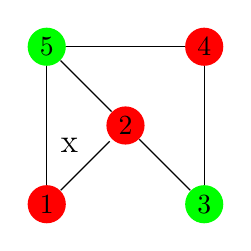
\begin{tikzpicture}[shorten >=1pt]
    \tikzstyle{vertex}=[circle,fill=black!25,minimum size=12pt,inner sep=2pt]
      \node[vertex,fill=red] (G_1) at (-1,-1) {1};
      \node[vertex,fill=red] (G_2) at (0,0)   {2};
      \node[vertex,fill=green] (G_3) at (1,-1)  {3};
      \node[vertex,fill=red] (G_4) at (1,1)   {4};
      \node[vertex,fill=green] (G_5) at (-1,1)  {5};
      \draw (G_1) -- node [midway, fill=white, yshift=7pt, xshift=-6pt] {\large x} (G_2);
      \draw (G_2) -- (G_3) -- cycle;
      \draw (G_1) -- (G_5) -- cycle;
      \draw (G_2) -- (G_5) -- cycle;
      \draw (G_5) -- (G_4) -- cycle;
      \draw (G_4) -- (G_3) -- cycle;
    \end{tikzpicture}
  }
};
\end{scope}
\end{tikzpicture} \\

\noindent Eine andere Art der Färbung besteht darin, allen Kanten Farben zuzuordnen auf eine Weise, dass Kanten, welche an der gleichen Ecke anliegen, nicht die gleiche Farbe haben. \\\\

\begin{tikzpicture}
\begin{scope}
  \node (0,0) {\parbox[c][40mm][c]{70mm}{\centering%
    Ein Beispiel dafür wäre:\\ \vspace{3mm}
    \begin{tikzpicture}[shorten >=1pt,->]
      \tikzstyle{vertex}=[circle,fill=black!25,minimum size=12pt,inner sep=2pt]
      \node[vertex] (G_1) at (-1,-1) {};
      \node[vertex] (G_2) at (0,0)   {};
      \node[vertex] (G_3) at (1,-1)  {};
      \node[vertex] (G_4) at (1,1)   {};
      \node[vertex] (G_5) at (-1,1)  {};
      \draw[red] (G_1) -- (G_2) -- cycle;
      \draw[green] (G_2) -- (G_3) -- cycle;
      \draw[green] (G_1) -- (G_5) -- cycle;
      \draw[blue] (G_2) -- (G_5) -- cycle;
      \draw[red] (G_5) -- (G_4) -- cycle;
      \draw[blue] (G_4) -- (G_3) -- cycle;
    \end{tikzpicture}
  }};
\end{scope}

\begin{scope}[xshift=75mm]
  \node (0,0) {\parbox[c][40mm][c]{70mm}{\centering%
  \noindent Ein Gegebeispiel dafür wäre\\ \vspace{3mm}
    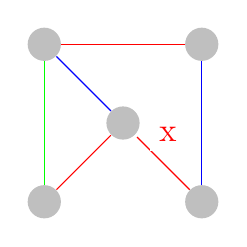
\begin{tikzpicture}[shorten >=1pt]
      \tikzstyle{vertex}=[circle,fill=black!25,minimum size=12pt,inner sep=2pt]
      \node[vertex] (G_1) at (-1,-1) {};
      \node[vertex] (G_2) at (0,0)   {};
      \node[vertex] (G_3) at (1,-1)  {};
      \node[vertex] (G_4) at (1,1)   {};
      \node[vertex] (G_5) at (-1,1)  {};
      \draw[red] (G_1) -- (G_2) -- cycle;
      \draw[red] (G_3) -- node [midway, fill=white, xshift=2pt, yshift=10pt] {\large x} (G_2);
      \draw[green] (G_1) -- (G_5) -- cycle;
      \draw[blue] (G_2) -- (G_5) -- cycle;
      \draw[red] (G_5) -- (G_4) -- cycle;
      \draw[blue] (G_4) -- (G_3) -- cycle;
    \end{tikzpicture}
  }
};
\end{scope}
\end{tikzpicture} \\

\subsection{Die Chromatische Zahl/Index}

Die Aufgabe, herauszufinden, was die minimale Anzahl von Farben ist, um einen Graphen zu färben, hat sich als äusserst schwierig erwiesen. Bis heute ist noch kein effizienter Algorithmus gefunden worden, um so ein Problem zu lösen. \\

\noindent \textbf{Chromatische Zahl} \\
Die kleinste Anzahl von Farben, welche benötigt wird, um die \textbf{Ecken} eines Graphen zu färben, nennt man die chromatische Zahl \(\chi\).\\
Für Menschen ist es jedoch ziemlich simpel, die effizienteste Färbung für einen sehr einfachen Graphen zu finden, wie hier illustriert wird. \\\\

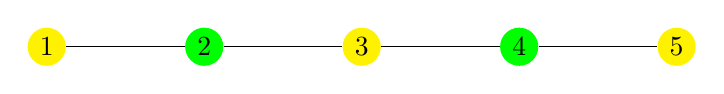
\begin{tikzpicture}[shorten >=1pt,->]
  \tikzstyle{vertex}=[circle,fill=black!25,minimum size=12pt,inner sep=2pt]
  \node[vertex,fill=yellow] (G_1) at (-4,0) {1};
  \node[vertex,fill=green] (G_2) at (-2,0)   {2};
  \node[vertex,fill=yellow] (G_3) at (0,0)  {3};
  \node[vertex,fill=green] (G_4) at (2,0)   {4};
  \node[vertex,fill=yellow] (G_5) at (4,0)  {5};
  \draw (G_1) -- (G_2) -- cycle;
  \draw (G_2) -- (G_3) -- cycle;
  \draw (G_3) -- (G_4) -- cycle;
  \draw (G_4) -- (G_5) -- cycle;
\end{tikzpicture} \\

\noindent Dieser Graph besitzt \(\chi = 2\), da ein Graph, der aus einer Linie von Ecken besteht, immer abwechselnd gefärbt werden kann. \\ \\

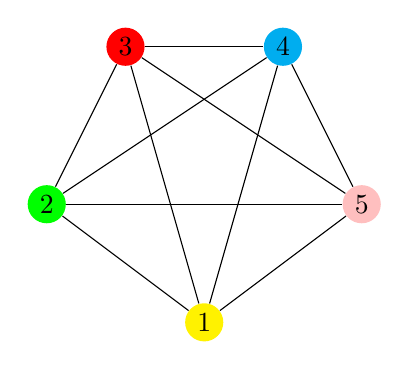
\begin{tikzpicture}[shorten >=1pt,->]
  \tikzstyle{vertex}=[circle,fill=black!25,minimum size=12pt,inner sep=2pt]
  \node[vertex,fill=yellow] (G_1) at (0,-1.5) {1};
  \node[vertex,fill=green] (G_2) at (-2,0)   {2};
  \node[vertex,fill=red] (G_3) at (-1,2)  {3};
  \node[vertex,fill=cyan] (G_4) at (1,2)   {4};
  \node[vertex,fill=pink] (G_5) at (2,0)  {5};
  \draw (G_1) -- (G_2) -- cycle;
  \draw (G_1) -- (G_3) -- cycle;
  \draw (G_1) -- (G_4) -- cycle;
  \draw (G_1) -- (G_5) -- cycle;
  \draw (G_2) -- (G_3) -- cycle;
  \draw (G_2) -- (G_4) -- cycle;
  \draw (G_2) -- (G_5) -- cycle;
  \draw (G_3) -- (G_4) -- cycle;
  \draw (G_3) -- (G_5) -- cycle;
  \draw (G_4) -- (G_5) -- cycle;
\end{tikzpicture} \\

\noindent Dieser Graph besitzt \(\chi=5\), da jede Ecke mit jeder anderen Ecke verbunden ist und jede Ecke damit eine andere Farbe haben muss. \\

\noindent \textbf{Chromatischer Index} \\
Die kleinste Anzahl von Farben, welche benötigt wird, um die \textbf{Kanten} eines Graphen zu färben, nennt man den chromatischen Index.\\
Der chromatische Index wird jedoch viel weniger in der Praxis verwendet als die chromatische Zahl.

\subsection{Reale Anwendung von Färbung}

Färbungen von Graphen werden oft verwendet, z.B. um Stundenpläne zu entwickeln, Ampeln effizient zu schalten etc. Alle diese Probleme werden in einen Graphen umgewandelt und dann gefärbt, wobei die chromatische Zahl die effizienteste Lösung für das Problem ist. \\

\noindent Die Herausforderung für uns ist es, das Problem als einen Graphen darzustellen. Hier werden oft Konfliktgrafen genutzt. Dabei sind die Ecken verschiedene Sachen, wie Lektionen, Tiere oder Fahrbahnen, und sie werden verbunden, wenn sie sich nicht vertragen und bei der Färbung dann nicht die gleiche Farbe haben können. \\

\noindent Nehme man die Personen Tom (T), Paul (P), Emma (E) und Gerald (G). Dabei vertragen sich aber Emma und Gerald, Tom und Gerald und Tom und Paul nicht. Dies kann wie gefolgt als ein Graph dargestellt werden. \\

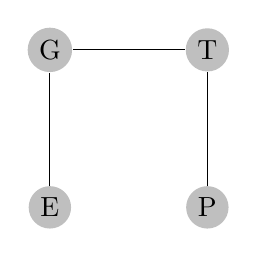
\begin{tikzpicture}[shorten >=1pt,->]
  \tikzstyle{vertex}=[circle,fill=black!25,minimum size=12pt,inner sep=2pt]
  \node[vertex] (T) at (1,1)   {T};
  \node[vertex] (P) at (1,-1)     {P};
  \node[vertex] (E) at (-1,-1)     {E};
  \node[vertex] (G) at (-1,1)      {G};
  \draw (E) -- (G) -- cycle;
  \draw (T) -- (G) -- cycle;
  \draw (T) -- (P) -- cycle;
\end{tikzpicture} \\

\noindent Die chromatische Zahl für diesen Graphen beträgt \(\chi=2\) und kann folgendermassen gefärbt werden \\
 
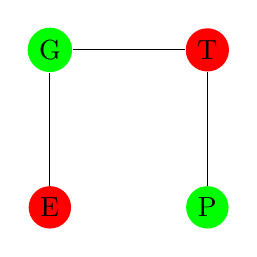
\begin{tikzpicture}[shorten >=1pt,->]
  \tikzstyle{vertex}=[circle,fill=black!25,minimum size=12pt,inner sep=2pt]
  \node[vertex,fill=red] (T) at (1,1)   {T};
  \node[vertex,fill=green] (P) at (1,-1)     {P};
  \node[vertex,fill=red] (E) at (-1,-1)     {E};
  \node[vertex,fill=green] (G) at (-1,1)      {G};
  \draw (E) -- (G) -- cycle;
  \draw (T) -- (G) -- cycle;
  \draw (T) -- (P) -- cycle;
\end{tikzpicture} \\

\noindent In diesem Fall können die Farben die Bedeutung tragen, dass sie einem Zimmer entsprechen, und somit haben wir gezeigt, dass Gerald und Paul in einem Zimmer sein können, wie auch Tom und Emma.

\subsection{Anzahl Färbungen / Chromatische Polynome}

Anstatt die optimale Färbung für einen Graphen zu finden, kann man sich auch die Frage stellen, wie viele Färbungen mit \(x\) Farben möglich sind. \\

\noindent Nehme man den folgenden Graphen, welcher mit \(x\) Farben gefärbt werden sollte. \\

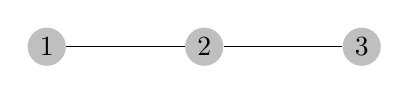
\begin{tikzpicture}[shorten >=1pt,->]
  \tikzstyle{vertex}=[circle,fill=black!25,minimum size=12pt,inner sep=2pt]
  \node[vertex] (G1) at (-2,0)  {1};
  \node[vertex] (G2) at (0,0)   {2};
  \node[vertex] (G3) at (2,0)   {3};
  \draw (G1) -- (G2) -- cycle;
  \draw (G2) -- (G3) -- cycle;
\end{tikzpicture} \\

\noindent Die Ecke 1 kann mit \(x\) Farben gefärbt werden, die zweite mit \((x-1)\) Farben, da eine Farbe schon aufgebraucht wurde. Die letzte Ecke darf dann nicht die Farbe der Ecke 2 haben, jedoch kann sie die Farbe der Ecke 1 haben, weshalb sie ebenfalls \((x-1)\) haben. \\

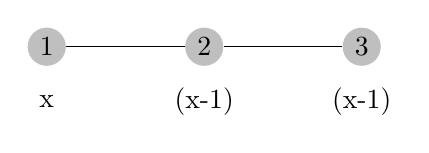
\begin{tikzpicture}[shorten >=1pt,->]
  \tikzstyle{vertex}=[circle,fill=black!25,minimum size=12pt,inner sep=2pt]
  \node[vertex] (G1) at (-2,0)  {1};
  \node at (-2, -0.7) {x};
  \node[vertex] (G2) at (0,0)   {2};
  \node at (0, -0.7) {(x-1)};
  \node[vertex] (G3) at (2,0)   {3};
  \node at (2, -0.7) {(x-1)};
  \draw (G1) -- (G2) -- cycle;
  \draw (G2) -- (G3) -- cycle;
\end{tikzpicture} \\

\noindent Damit gibt es für \(x\) Farben \(x(x-1)^2\) verschiedene Färbungen, dieses Polynom wird auch chromatisches Polynom genannt. Für einen Graphen \(G\) wird die Funktion, welche das chromatische Polynom berechnet, \(F(G)\) gennant. \\

\noindent Ein weiteres Beispiel mit dem folgenden Graph \\

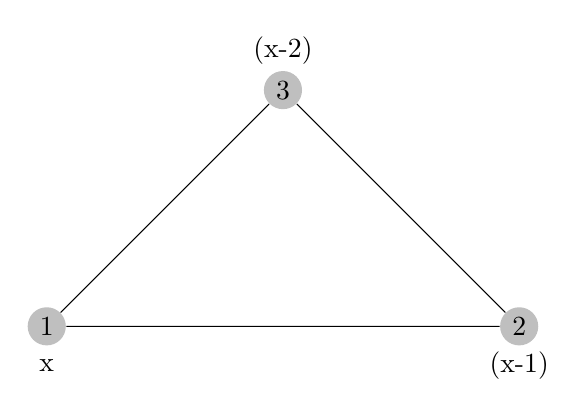
\begin{tikzpicture}[shorten >=1pt,->]
  \tikzstyle{vertex}=[circle,fill=black!25,minimum size=12pt,inner sep=2pt]
  \node[vertex] (G1) at (-3,-1)   {1};
  \node at (-3, -1.5) {x};

  \node[vertex] (G2) at (3,-1)    {2};
  \node at (3, -1.5) {(x-1)};

  \node[vertex] (G3) at (0,2)   {3};
  \node at (0, 2.5) {(x-2)};

  \draw (G1) -- (G2) -- (G3) -- (G1) -- cycle;
\end{tikzpicture} \\

\noindent Welcher das chromatische Polynom \(x(x-1)(x-2)\) besitzt. \\

\noindent Der folgende Graph wird ein Baum genannt, weil der Graph aus einer Ecke (Stamm) herauswächst zu weiteren Ecken (Äste).

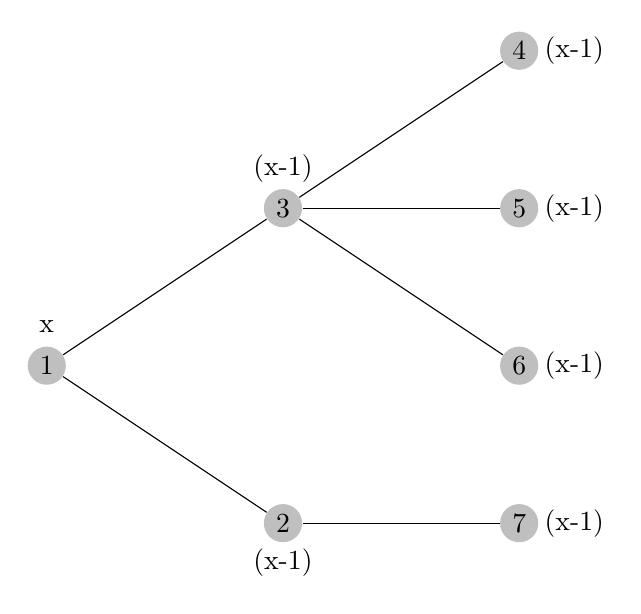
\begin{tikzpicture}[shorten >=1pt,->]
  \tikzstyle{vertex}=[circle,fill=black!25,minimum size=12pt,inner sep=2pt]
  \node[vertex] (G1) at (0,0)   {1};
  \node[vertex] (G2) at (3,-2)  {2};
  \node[vertex] (G3) at (3,2)   {3};
  \node[vertex] (G4) at (6,4)   {4};
  \node[vertex] (G5) at (6,2)   {5};
  \node[vertex] (G6) at (6,0)   {6};
  \node[vertex] (G7) at (6,-2)  {7};

  \node at (0, 0.5) {x};
  \node at (3, 2.5) {(x-1)};
  \node at (3, -2.5) {(x-1)};
  \node at (6.7, 4) {(x-1)};
  \node at (6.7, 2) {(x-1)};
  \node at (6.7, 0) {(x-1)};
  \node at (6.7, -2) {(x-1)};

  \draw (G1) -- (G2) -- cycle;
  \draw (G1) -- (G3) -- cycle;
  \draw (G2) -- (G7) -- cycle;
  \draw (G3) -- (G4) -- cycle;
  \draw (G3) -- (G5) -- cycle;
  \draw (G3) -- (G6) -- cycle;
\end{tikzpicture} \\

\noindent Damit ist das chromatische Polynom dieses Graphen \(x(x-1)^6\). \\

\noindent Ein Graph, bei welchem jede Ecke mit jeder anderen Ecke verbunden ist, nennt sich ein n-Eck, wobei er \(n\) Ecken beinhaltet. Sein chromatisches Polynom für \(x\) Farben ist \(x(x-1)(x-2) \cdots (x-(n-1))\)

\subsection{Algorithmus für das chromatische Polynom}

Der Algorithmus besteht aus den folgenden Schritten und basiert darauf, das Problem rekursiv zu vereinfachen, für Graphen, für welche das chromatische Polynom bekannt ist.

\begin{itemize}
    \item Wähle eine beliebige Kante aus einem Graphen \(G\) aus
    \item Kopiere den Graph \(G\) und lösche diese Kante in dem kopierten Graph \(G_1\)
    \item Kopiere den graph \(G\) und \textit{ziehe} diese Kante zusammen in dem kopierten Graph \(G_2\)
    \item Ist bekannt, wie viele Färbungen die Graphen \(G_1\) und \(G_2\) haben?
    \begin{itemize}
      \item \textbf{Ja}: Die Lösung ist \(F(G)=F(G_1) - F(G_2)\)
      \item \textbf{Nein}: Wiederhole das Verfahren für \(G_1\) und \(G_2\)
    \end{itemize}
\end{itemize}

\noindent Die kleinste Lösung für das Polynom, welche positiv ist, sodass es immer noch positiv ist, ist die chromatische Zahl!

\subsection{Beweise auf Graphen}

Für Beweise auf Graphen wird oft die mathematische Induktion benutzt. Hier eine kurze Erinnerung an die Induktion. \\
\noindent Die Induktion ist oft nützlich für Hypothesen, welche eine Variable beinhalten, welche eine natürliche Zahl ist, wie die Anzahl (\(n\)) von Ecken in einem Graph. Dann wird die Aussage für ein n bewiesen, wie \(n=0\) bzw. einen Graph mit 0 Ecken. Im Induktionsschritt wird dann die Aussage für \(n\) als wahr angenommen und man probiert zu zeigen, dass die Aussage auch für \(n+1\) stimmt.\\

\noindent \textbf{Hypothese:} Sei \(g_{max}\) der höchste Grad einer Ecke in einem einfachen Graph, so ist die chromatische Zahl höchstens \(g_{max}+1\) \\

\noindent \textbf{Beweis} \\ 
\noindent Zuerst müssen, wir unsere Hypothese umwandeln, dass sie ein \(n\) beinhaltet.\vspace{1mm} \\ 
\noindent \textbf{Induktionshypothese} Sei \(g_{max}\) der höchste Grad einer Ecke in einem einfachen Graphen mit \(n\) Ecken, so ist die chromatische Zahl höchstens \(g_{max}+1\) \vspace{1mm} \\
\noindent \textbf{Induktionsanfang} Zu zeigen ist, dass die Aussage für \(n=1\) stimmt, was wir sofort sehen, da ein einfacher Graph mit nur einer Ecke keine Kanten haben kann und deshalb ist \(g_{max}=0\) und man braucht nur eine Farbe, um eine Ecke zu färben, was grösser oder gleich \(g_{max}+1\) ist.  \vspace{1mm} \\
\noindent \textbf{Induktionsschritt:} Nehme die Aussage für \(n\) an, um \(n+1\) zu zeigen. \\ 
Nehme man einen Graphen \(G_1\) mit \(n+1\) Ecken, dann kann eine Ecke \(k\) mit allen ihren Kanten entfernt werden. Wir erhalten damit einen einfachen Graphen \(G_2\) mit \(n\) Ecken, auf welchen wir unsere Induktionshypothese anwenden können. \\
Wir wissen, dass ein Graph mit \(g_{max}+1\) Farben gefärbt werden kann, wenn \(g_{max}\) der höchste Grad einer Ecke im Graph \(G_2\) ist. Wenn wir die Ecke \(k\) mit allen ihren Kanten einfügen, ergeben sich zwei Fälle.

\begin{itemize}
  \item \(g_{max}\) wird erhöht, dann kann eine neue Farbe verwendet werden für \(k\).
  \item \(g_{max}\) wird nicht erhöht, dann gehen weniger als \(g_{max}\) Kanten in die Ecke \(k\) hinein, weshalb eine Farbe immer noch frei ist von den \(g_{max}\) Farben für die Ecke \(k\). 
\end{itemize}

\end{document}

